%% This is file AJCEAM-paper.tex is the template file for publications
%% in the "Academic Journal on Computing, Engineering and Applied Mathematics
%% from Universidade Federal do Tocatins, Brazil,
%% https://sistemas.uft.edu.br/periodicos/index.php/AJCEAM/index
%% This file was originally written by Tiago Almeida.
%% First revision: 2019-10-29
%% Second revision:
%%
%% History:
%%           2019-10-29 - First version by Tiago Almeida <tiagoalmeida@uft.edu.br>.
%%           2020-04-09 - English revision by Caio Machado <caio.machado@uft.edu.br>
%%

% Options
%     eng:   English Language
%     por:   Portuguese Language
%     blind: The version for reviewers is compiled (author data is hidden)


\documentclass[eng]{ajceam-class}
%
% Publication Title
\title{Kalman Filter Research}

% Publication Title (Portuguese only)
% \titulo{Instruções para os autores da Academic Journal on Computing, Engineering and Applied Mathematics}

% Short title for the header (copy the main title if it is not too long)
% \shorttitle{Author instructions for the AJCEAM}
       
% Authors
\author[1]{Pengfei Nie}
% \author[2]{Name B. Surname}
% \author[1,2,3]{Name C. Surname}

% Author Affiliations
\affil[1]{V2X Software Engineer & pfnie@yahoo.com & https://github.com/pengfeinie}
% \affil[2]{(Other) University Name, Department Name or Institute, State, Country}
% \affil[3]{(Other) University Name, Department Name or Institute, State, Country}

% % Surname of the first author of the manuscript
% \firstauthor{SurnameA, SurnameB and SurnameC}

% %Contact Author Information
% \contactauthor{Name A. Surname}           % Name and surname of the contact author
% \email{name.surname@email.com} % Contact Author Email

% Publication data (will be defined in the edition)
 \thisvolume{20221006}
% \thisnumber{XX}
% \thismonth{Month}
% \thisyear{20XX}
% \receptiondate{dd/mm/aaaa}
% \acceptancedate{dd/mm/aaaa}
 \publicationdate{20221006}
% \receptiondate{08/10/2022}
% \acceptancedate{08/10/2022}

% Place your particular definitions here
\newcommand{\vect}[1]{\mathbf{#1}}  % vectors

% Insert here the abstract in English language
\abstract{
Most modern systems have numerous sensors that estimate hidden (unknown) states based on a series of measurements.the measurement uncertainty depends on many external factors.The Kalman Filter is one of the most important and common estimation algorithms. The Kalman Filter produces estimates of hidden variables based on inaccurate and uncertain measurements. Also, the Kalman Filter predicts the future system state based on past estimations.The filter is named after Rudolf E. Kálmán (May 19, 1930 – July 2, 2016). In 1960, Kálmán published his famous paper describing a recursive solution to the discrete-data linear filtering problem.}

% Insert here the keywords of your work in English language
\keywords{
Kalman Filter, Measurements, Estimation Algorithms , Prediction.}


% % Insert here the abstract in Portuguese language
% \resumo{
% Este documento fornece um modelo para a elaboração de trabalhos originais cujos autores desejam ser publicados na Academic Journal on Computing, Engineering and Applied Mathematics da Universidade Federal do Tocantins Tocantins, Brasil. A princípio, recomendamos fortemente que o resumo seja escrito em um único parágrafo contendo no mínimo 150 e no máximo 200 palavras. Nesta seção de texto, espera-se um resumo incluindo o contexto, motivação, metodologia, as contribuições mais originais, resultados e conclusões do seu trabalho. Além disso, citações bibliográficas, siglas ou fórmulas devem ser evitadas tanto no resumo quanto no título. Também é fortemente recomendado evitar quaisquer referências a figuras ou tabelas nesta seção. Finalmente, é uma boa prática escrever seu artigo inserindo texto e excluindo diretamente deste arquivo de modelo para manter os estilos predefinidos.}

% Insert here the keywords of your work in Portuguese language
% \palavraschave{
% Primeira palavra ou frase-chave, segunda palavra ou frase-chave, terceira palavra ou frase-chave. (Coloque entre três e seis palavras-chave ou frases separadas por vírgula, que representam o tema do seu trabalho)}

% Start document
\begin{document}

% Include title, authors, abstract, etc.
\maketitle
\thispagestyle{fancy}
% \printcontactdata

% Main body of manuscript
\section{Introduction}
\quad In statistics and control theory, Kalman filtering, also known as linear quadratic estimation, is an algorithm that uses a series of measurements observed over time, containing statistical noise and other inaccuracies, and produces estimates of unknown variables that tend to be more accurate than those based on a single measurement alone, by estimating a joint probability distribution over the variables for each timeframe. The filter is named after Rudolf E. Kálmán, one of the primary developers of its theory.

The algorithm works in a two-step process. In the prediction step, the Kalman filter produces estimates of the current state variables, along with their uncertainties. Once the outcome of the next measurement (necessarily corrupted with some amount of error, including random noise) is observed, these estimates are updated using a weighted average, with more weight being given to estimates with higher certainty. The algorithm is recursive. It can run in real time, using only the present input measurements and the previously calculated state and its uncertainty matrix; no additional past information is required.

Extensions and generalizations to the method have also been developed, such as the extended Kalman filter and the unscented Kalman filter which work on nonlinear systems. The underlying model is a hidden Markov model where the state space of the latent variables is continuous and all latent and observed variables have Gaussian distributions. Also, the Kalman filter has been successfully used in multi-sensor fusion, and distributed sensor networks to develop distributed or consensus Kalman filter.
\section{weight the gold}
Now we are ready for the first simple example. In this example, we estimate a static system's state. A static system is a system that doesn't change its state over a reasonable period. For instance, the static system could be a tower, and the state would be its height.
In this example, we estimate a gold bar's weight. But the measurements do include random noise.The system is the gold bar, and the system's state is the weight of the gold bar. The system's dynamic model is constant since we assume that the weight doesn't change over short periods.
In order to estimate the system's state (i.e., the weight value), we can make multiple measurements and average them.
\subsection{Estimate The Weight of Gold}

$$
\centering
\includegraphics[width=.9\columnwidth]{gold_weight.png} 
$$
$$
\hat{x}_{n, n}=\frac{1}{n}\left(z_1+z_2+\ldots+z_{n-1}+z_n\right)=\frac{1}{n} \sum_{i=1}^n\left(z_i\right)
$$
\begin{table}[!b]
 \centering
  \caption{Example Notation} \label{table-1}
 {\small
 \begin{tabular}{ccccc}
  \hline
  \hline
  \thead{variables} & \thead{description} \\
  \hline
  \hline
  $x$ & is the true value of the weight. \\
  \hline
  $z_n$ & is the measured value of the weight at time $n$. \\
  \hline
$\hat{x}_{n, n}$ & is the estimate of $x$ at time $n$. \\
  \hline
  \hline
$\hat{x}_{n+1, n}$ & is the predicted of the future state $(n+1)$ of $x$.\\
  \hline
 $\hat{x}_{n-1, n-1}$ & is the estimate of $x$ at time $n-1$. \\
  \hline
 $\hat{x}_{n, n-1}$ & is the predicted of the future state $n$ of $x$.\\
  \hline
  \hline
 \end{tabular}}
\end{table}

\begin{aligned}
&\hat{x}_{n, n}=\frac{1}{n} \sum_{i=1}^n\left(z_i\right) \\
&=\frac{1}{n}\left(\sum_{i=1}^{n-1}\left(z_i\right)+z_n\right) \\
&=\frac{1}{n} \sum_{i=1}^{n-1}\left(z_i\right)+\frac{1}{n} z_n \\
&=\frac{1}{n} \frac{n-1}{n-1} \sum_{i=1}^{n-1}\left(z_i\right)+\frac{1}{n} z_n \\
&=\frac{n-1}{n} \frac{1}{n-1} \sum_{i=1}^{n-1}\left(z_i\right)+\frac{1}{n} z_n \\
&=\frac{n-1}{n} \hat{x}_{n-1, n-1}+\frac{1}{n} z_n \\
&=\hat{x}_{n-1, n-1}-\frac{1}{n} \hat{x}_{n-1, n-1}+\frac{1}{n} z_n \\
&=\hat{x}_{n-1, n-1}+\frac{1}{n}\left(z_n-\hat{x}_{n-1, n-1}\right)\\
\end{aligned}\\
\\
Since the dynamic model in this example is static, i.e., the weight of the gold bar doesn't change over time, the predicted state of $x$ equals the estimated state of $x$ :
$$
\hat{x}_{n, n-1}=\hat{x}_{n-1, n-1}
$$
Based on the above, the estimate of the current state $\hat{x}_{n, n}$, can be written as follows:\\
$$
\hat{x}_{n, n}=\hat{x}_{n, n-1}+\frac{1}{n}\left(z_n-\hat{x}_{n, n-1})
$$

The factor $\frac{1}{n}$ is specific for our example. We will discuss the vital role of this factor later.The subscript $n$ indicates that the it can change with every iteration.

The term $\left(z_n-\hat{x}_{n, n-1})$ is the "measurement residual".In this example, $\frac{1}{n}$ decreases as $n$ increases. In the beginning, we don't have enough information about the current state; thus, the first estimation is based on the first measurement $\left.\frac{1}{n}\right|_{n=1}=1$. As we continue, each successive measurement has less weight in the estimation process, since $\frac{1}{n}$ decreases.
Let's continue with the example. Before we make the first measurement, we can guess (or rough estimate) the gold bar weight simply by reading the stamp on the gold bar. It is called the Initial Guess, and it is our first estimate.
The Kalman Filter requires the initial guess as a preset, which can be very rough.

\subsubsection{Zero Iteration}
\textbf{Initialization}\\
Our initial guess of the gold bar weight is 1000 grams. The initial guess is used only once for the filter initiation. Thus, it won't be required for success iterations.
$$
\hat{x}_{0,0}=1000 g
$$
\textbf{Prediction}\\
The weight of the gold bar is not supposed to change. Therefore, the dynamic model of the system is static. Our next state estimate (prediction) equals the initialization:
$$
\hat{x}_{1,0}=\hat{x}_{0,0}=1000 g
$$
\subsubsection{First Iteration}
\textbf{Step 1}\\
Making the weight measurement with the scales:
$$
{z}_{1}=1030 g
$$
\textbf{Step 2}\\
Calculating the factor,thus:
$$
\frac{1}{n}=\frac{1}{1}=1
$$
Calculating the current estimate State:
$$
\hat{x}_{1, 1}=\hat{x}_{1, 0}+\frac{1}{1}\left(z_1-\hat{x}_{1, 0}\right)=1000+1(1030-1000)=1030g
$$
\textbf{Step 3}\\
The dynamic model of the system is static; thus, the weight of the gold bar is not supposed to change. Our next state prediction equals to current state estimate:
$$
\hat{x}_{2,1}=\hat{x}_{1,1}=1030 g
$$
\subsubsection{Second Iteration}
After a unit time delay, the predicted estimate from the previous iteration becomes the previous estimate in the current iteration:
$$
\hat{x}_{2,1}=1030 g
$$
\textbf{Step 1}\\
Making the second measurement of the weight:
$$
{z}_{1}=989 g
$$
\textbf{Step 2}\\
Calculating the factor,thus:
$$
\frac{1}{n}=\frac{1}{2}
$$
Calculating the current estimate State:
$$
\hat{x}_{2, 2}=\hat{x}_{2, 1}+\frac{1}{2}\left(z_2-\hat{x}_{2, 1}\right)=1030+\frac{1}{2}(989-1030)=1009.5g
$$

\textbf{Step 3}\\
The dynamic model of the system is static; thus, the weight of the gold bar is not supposed to change. Our next state prediction equals to current state estimate:
$$
\hat{x}_{3,2}=\hat{x}_{2,2}=1009.5g
$$
We can stop here. The gain decreases with each measurement. Therefore, the contribution of each successive measurement is lower than the contribution of the previous measurement. We get pretty close to the true weight, which is 1010g. If we were making more measurements, we would get closer to the true value.

The following table summarizes our measurements and estimates, and the chart compares the measured values, the estimates, and the true value.
$$
\centering
\includegraphics[width=.9\columnwidth]{gold_10_graph} 
$$
\section{Estimate The State of Aircraft }
\subsection{Tracking Constant Velocity Air in One Dimension}
It is time to examine a dynamic system that changes its state over time.Let us assume a one-dimensional world. We assume an aircraft that is moving radially away from the radar. In the one-dimensional world, the angle to the radar is constant, and the aircraft's altitude is constant, as shown in the following figure.
$$
\centering
\includegraphics[width=.9\columnwidth]{air} 
$$
${x}_{n}$ represents the range to the aircraft at time ${n}$. The aircraft velocity can be approximated using the range differentiation method - the change in the measured range with time. Thus, the velocity is a derivative of the range:
$$
{v} = \frac{dx}{dt}
$$
The radar sends a track beam in the direction of the target at a constant rate. The track-to-track interval is ${\Delta t}$.
Two equations of motion can describe the system's dynamic model for constant velocity motion:
$$
{x}_{n+1} = {x}_{n} + {\Delta t}*{v}
$$
$$
{v}_{n+1} = {v}_{n}
$$
According to these equations, the aircraft range at the next track cycle equals the range at the current track cycle plus the target velocity multiplied by the track-to-track interval. Since we assume constant velocity in this example, the velocity at the next cycle equals the velocity at the current cycle.
This system of equations extrapolates the current state to the next state.The Equations depend on the system dynamics and differ from example to example.
\subsubsection{The ${\alpha - \beta}$ Filter}
Let the radar track-to-track ( ${\Delta t}$ period be 5 seconds. Assume that at time ${n}-{1}$ the estimated range of the aircraft is 30,000m, and the estimated aircraft velocity is 40m/s. \\
Using the above Equations, we can predict the target position at time ${n}$ :
$$
\hat{x}_{n,n-1} = \hat{x}_{n-1,n-1} + {\Delta t}*\hat{v}_{n-1,n-1}=30000+{5}*40=30200m
$$
The target velocity prediction for time ${n}$:
$$
\hat{v}_{n,n-1} = \hat{v}_{n-1,n-1} = 40m/s
$$
However, at time n, the radar measures range ( ${z}_{n}$ ) of 30,110m and not 30,200m as expected. There is a 90m gap between the predicted range and the measured range. There are two possible reasons for this gap:
\begin{itemize}
    \item The radar measurements are not precise.
    \item The aircraft velocity has changed. The new aircraft
    
    velocity is:
    $\frac{30,110-30,000}{5}$ = 22m/s
\end{itemize}
Which of the two statements is true?
Let us write down the Equation for the velocity:
$$
\hat{v}_{n,n} = \hat{v}_{n,n-1} + {\beta}(\frac{{z}_{n} - \hat{x}_{n,n-1}}{\Delta t})
$$
The value of the factor ${\beta}$ depends on the precision level of the radar. Suppose that the 1${\sigma}$ precision of the radar is 20m. The 90 meters gap between the predicted and measured ranges most likely results from a change in the aircraft velocity. We should set the ${\beta}$ factor to a high value in this case. If we set ${\beta}$ = 0.9, then the estimated velocity would be:
$$
\hat{v}_{n,n} = \hat{v}_{n,n-1} + {\beta}(\frac{{z}_{n} - \hat{x}_{n,n-1}}{\Delta t})
$$
$$
&=40+0.9(\frac{30,110 - 30,200}{5})=23.8m/s
$$

On the other hand, suppose that the 1${\sigma}$ precision of the radar is 150m. Then the 90 meters gap probably results from the radar measurement error. We should set the ${\beta}$ factor to a low value in this case. If we set ${\beta}$ = 0.1, then the estimated velocity would be:
$$
\hat{v}_{n,n} = \hat{v}_{n,n-1} + {\beta}(\frac{{z}_{n} - \hat{x}_{n,n-1}}{\Delta t})
$$
$$
&=40+0.1(\frac{30,110 - 30,200}{5})=38.2m/s
$$
If the gap has been caused by measurement error, then the successive measurements would be in front or behind the predicted positions. Thus on average, the target velocity would not change.\\

The Equation for the aircraft position:
$$
\hat{x}_{n,n} = \hat{x}_{n,n-1} + {\alpha}({z}_{n} - \hat{x}_{n,n-1})
$$
The magnitude of the ${\alpha}$ factor depends on the radar measurement precision. For high precision radar, we should choose high ${\alpha}$, giving high weight to the measurements.\\
If ${\alpha}$=1, then the estimated range equals the measured range:
$$
\hat{x}_{n,n} = \hat{x}_{n,n-1} + 1({z}_{n} - \hat{x}_{n,n-1})={z}_{n}
$$
If ${\alpha}$=0 , then the measurement has no meaning:
$$
\hat{x}_{n,n} = \hat{x}_{n,n-1} + 0({z}_{n} - \hat{x}_{n,n-1})=\hat{x}_{n,n-1}
$$
So, we have derived a system of equations that composes the Equation for the radar tracker.

$$
\hat{x}_{n,n} = \hat{x}_{n,n-1} + {\alpha}({z}_{n} - \hat{x}_{n,n-1})
$$
$$
\hat{v}_{n,n} = \hat{v}_{n,n-1} + {\beta}(\frac{{z}_{n} - \hat{x}_{n,n-1}}{\Delta t})
$$
\\
The following chart depicts the true values, measured values, and estimates for ${\alpha}=0.2$ and ${\beta}=0.1$.
$$
\centering
\includegraphics[width=.9\columnwidth]{air_low_factor} 
$$
The following chart depicts the true values, measured values, and estimates for ${\alpha}=0.8$ and ${\beta}=0.5$.
$$
\centering
\includegraphics[width=.9\columnwidth]{air_high_factor} 
$$
The "smoothing" degree of this filter is much lower. The "current estimate" is very close to the measured values, and predicted estimate errors are pretty high.

So, shall we always choose low values for ${\alpha}$ and ${\beta}$ ?

The answer is NO. The value of ${\alpha}$ and ${\beta}$ should depend on the measurement precision. If we use high precision equipment, like laser radar, we would prefer a high ${\alpha}$ and ${\beta}$ that follow measurements. In this case, the filter would quickly respond to a velocity change of the target. On the other hand, if measurement precision is low, we prefer low ${\alpha}$ and ${\beta}$. In this case, the filter smoothes the uncertainty (errors) in the measurements. However, the filter reaction to target velocity changes would be much slower.

\subsection{Tracking Accelerating Air in One Dimension}
\subsubsection{The ${\alpha - \beta - \gamma}$ Filter}
Thus, the State Extrapolation Equations become:
$$
\hat{x}_{n,n-1} = \hat{x}_{n-1,n-1} + \hat{v}_{n-1,n-1}{\Delta t} + \hat{a}_{n-1,n-1}\frac{{\Delta t^2}}{2}
$$
$$
\hat{v}_{n,n-1} = \hat{v}_{n-1,n-1} + \hat{a}_{n-1,n-1}{\Delta t}
$$
$$
\hat{a}_{n,n-1} = \hat{a}_{n-1,n-1}
$$
The State Update Equations become:
$$
\hat{x}_{n,n} = \hat{x}_{n,n-1} + {\alpha}({z}_{n} - \hat{x}_{n,n-1})
$$
$$
\hat{v}_{n,n} = \hat{v}_{n,n-1} + {\beta}(\frac{{z}_{n} - \hat{x}_{n,n-1}}{\Delta t})
$$
$$
\hat{a}_{n,n} = \hat{a}_{n,n-1} + {\gamma}(\frac{{z}_{n} - \hat{x}_{n,n-1}}{0.5\Delta t^2})
$$
Let's take the scenario from the example: an aircraft that moves with a constant velocity of 50m/s for 15 seconds and then accelerates with a constant acceleration of 8m/s2 for another 35 seconds.
The ${\alpha - \beta - \gamma}$ filter parameters are:

\begin{itemize}
\item ${\alpha = 0.5}$
\item ${\beta = 0.4}$
\item ${\gamma = 0.1}$
\end{itemize}
The track-to-track interval is 5 seconds.
$$
\centering
\includegraphics[width=.9\columnwidth]{air_3_1} 
$$
$$
\centering
\includegraphics[width=.9\columnwidth]{air_3_2} 
$$
$$
\centering
\includegraphics[width=.9\columnwidth]{air_3_3} 
$$

As you can see, the ${\alpha - \beta - \gamma}$ filter with dynamic model equations that include acceleration can track the target with constant acceleration. 

But what happens in the case of a maneuvering target? The target can suddenly change the flight direction by making a maneuver. The target's dynamic model can also include a changing acceleration. In such cases, the ${\alpha - \beta - \gamma}$ filter with constant ${\alpha - \beta - \gamma}$ coefficients produces estimation errors and, in some cases, loses the target track.

The Kalman filter can handle uncertainty in the dynamic model.

\section{Kalman filter}
\subsection{State Extrapolation Equation}
Until now, we've dealt with one dimensional processes, like estimating the liquid temperature. But many dynamic processes have two, three, or even more dimensions.

\textbf{Airplane - No Control Input}

For instance, the state vector that describes the airplane's position in space is one-dimensional. The state vector that describes the airplane position and velocity is two-dimensional.
The state vector that describes the airplane position, velocity, and acceleration is three-dimensional.
$$
\left[\begin{array}{c}
x \\
\dot{x} \\
\ddot{x} \\
\end{array}\right]\\
$$
\\
Assuming a constant acceleration dynamic model, we can describe the extrapolated airplane state at time n by nine motion equations:
\\

\left\{\begin{array}{l}
\hat{x}_{n,n-1}=\hat{x}_{n-1,n-1}+\hat{\dot{x}}_{n-1,n-1} \Delta t+\frac{1}{2} \hat{\ddot{x}}_{n-1,n-1} \Delta t^{2} \\
\hat{\dot{x}}_{n,n-1}=\hat{\dot{x}}_{n-1,n-1}+\hat{\ddot{x}}_{n-1,n-1} \Delta t \\
\hat{\ddot{x}}_{n,n-1}=\hat{\ddot{x}}_{n-1,n-1} \\
\end{array}\right.
\\

$$
\left[\begin{array}{c}
\hat{x}_{n, n-1} \\
\hat{\dot{x}}_{n, n-1} \\
\hat{\ddot{x}}_{n, n-1} \\
\end{array}\right]=\left[\begin{array}{ccccccccc}
1 &  & \Delta t &  &   0.5 \Delta t^{2}   \\
0 &  &   1 &  &   \Delta t   \\
0 &  &   0 &  &   1   \\
\end{array}\right]\left[\begin{array}{l}
\hat{x}_{n-1, n-1} \\
\hat{\dot{x}}_{n-1, n-1} \\
\hat{\ddot{x}}_{n-1, n-1} \\
\end{array}\right]
$$

It is common practice to describe a multidimensional process with a single equation in matrix form.First, it is very exhausting to write all these equations; representing them in matrix notation is much shorter and more elegant.Second, computers are highly efficient at matrix calculations. Implementing the Kalman Filter in matrix form yields faster computation run time.

The following chapters describe the Kalman Filter equations in matrix form. And, of course, the theoretical part is followed by fully solved numerical examples.
\\
The state extrapolation equation is:
$$
\hat{x}_{n,n-1} = {F}\hat{x}_{n-1,n-1} 
$$
\\
\textbf{Airplane - With Control Input}\\
This example is similar to the previous example, but now we have a sensor connected to the pilot's controls, so we have additional information about the airplane acceleration based on the pilot's commands.

$$
\left[\begin{array}{c}
x \\
\hat{\dot{x}} \\
\end{array}\right]\\
$$
\\
The control vector that describes the measured airplane acceleration in a cartesian coordinate system is:
$$
\left[\begin{array}{c}
\hat{\ddot{x}} \\
\end{array}\right]\\
$$
\\
\left\{\begin{array}{l}
\hat{x}_{n,n-1}=\hat{x}_{n-1,n-1}+\hat{\dot{x}}_{n-1,n-1} \Delta t+\frac{1}{2} {\ddot{x}_{n-1,n-1} \Delta t^{2} \\
\hat{\dot{x}}_{n,n-1}=\hat{\dot{x}}_{n-1,n-1}+{\ddot{x}}_{n-1,n-1} \Delta t \\
\end{array}\right.



$$
\left[\begin{array}{c}
\hat{x}_{n, n-1} \\
\hat{\dot{x}}_{n, n-1} \\
\end{array}\right]=\left[\begin{array}{ccccccccc}
1 &  \Delta t \\
0 & 1  \\
\end{array}\right]\left[\begin{array}{l}
\hat{x}_{n-1, n-1} \\
\hat{\dot{x}}_{n-1, n-1} \\
\end{array}\right]+\left[\begin{array}{ccccccccc}
\frac{1}{2}\Delta t^2 \\
\Delta t  \\
\end{array}\right]\left[\begin{array}{l}
{\ddot{x}}_{n-1, n-1} \\
\end{array}\right]
$$

The state extrapolation equation is:
$$
\hat{x}_{n,n-1} = {F}\hat{x}_{n-1,n-1} + {G}{u}_{n-1,n-1}
$$
\\
\textbf{Falling Object - With Control Input}\\
Consider a free-falling object. The state vector includes the altitude ${h}$ and the object's velocity ${v}$: 
$$
\left[\begin{array}{c}
{h} \\
{v} \\
\end{array}\right]\\
$$
\\
The equation  results in: 
\\
$$
\left\{\begin{array}{l}
\hat{h}_{n,n-1}=\hat{h}_{n-1,n-1}+\Delta t \hat{v}_{n-1,n-1} +\frac{1}{2} \Delta t^{2}{g} \\
\hat{v}_{n,n-1}=\hat{v}_{n-1,n-1}+\Delta t{g} \\
\end{array}\right.
\\
$$
Where ${g}$ is the gravitational acceleration.
We don't have a sensor that measures acceleration, but we know that for a falling object, acceleration equals ${g}$.The state extrapolation equation looks as follows:
\\
$$
\left[\begin{array}{l}
\hat{h}_{n, n-1} \\
\hat{v}_{n, n-1}
\end{array}\right]=\left[\begin{array}{cc}
1 & \Delta t \\
0 & 1
\end{array}\right]\left[\begin{array}{l}
\hat{h}_{n-1, n-1} \\
\hat{v}_{n-1, n-1}
\end{array}\right]+\left[\begin{array}{c}
0.5 \Delta t^{2} \\
\Delta t
\end{array}\right][g]
\\
$$
The state extrapolation equation is:
$$
\hat{x}_{n,n-1} = {F}\hat{x}_{n-1,n-1} + {G}{u}_{n-1,n-1}
$$
\textbf{Summary}\\
Using the state extrapolation equation, we can predict the next system state based on the knowledge of the current state. It extrapolates the state vector from the present (time step ${n-1}$ ) to the future (time step ${n}$ ). Extrapolation is the method of predicting the value of the independent variable for a certain value of the dependent variable outside of the available data set using suitable mathematical tools and models.

\begin{equation} \label{ec-1}
\hat{x}_{n,n-1} = {F}\hat{x}_{n-1,n-1} + {G}{u}_{n-1,n-1} + {w}_{n-1,n-1}
\end{equation}

The following table specifies the matrix dimensions of the state extrapolation equation variables: 
\begin{table}[!b]
 \centering
  \caption{Example Notation} \label{table-1}
 {\small
 \begin{tabular}{ccccc}
  \hline
  \hline
  \thead{variables} & \thead{description} \\
  \hline
  \hline
  $\hat{x}_{n,n-1}$ & is a predicted system state vector at time step ${n}$. \\
  \hline
  $\hat{x}_{n-1,n-1}$ & is a estimated system state vector at time step ${(n-1)}$. \\
  \hline
${u}_{n-1, n-1}$ & is a control variable at time $(n-1)$. \\
  \hline
${w}_{n-1, n-1}$ & is a process noise $(n-1)$.\\
  \hline
 $F$ & is a state transition matrix. \\
  \hline
 $G$ & is a control matrix. \\
  \hline
  \hline
 \end{tabular}}
\end{table}


\subsection{Covariance Extrapolation Equation}
Assume vector ${x}$ with ${k}$ elements:
$$
{x}=\left[\begin{array}{c}
{x}_{1} \\
{x}_{2} \\
{.}\\
{.}\\
{.}\\
{x}_{k}\\
\end{array}\right]\\
$$
The covariance matrix of the vector ${x}$ is given by:
$$
{Cov(x)}={E}(({x}-{\mu}_{x})({x}-{\mu}_{x})^T)
$$

$$
M=\left[\begin{array}{ccccc}
a_{11} & a_{12} & a_{13} & \cdots & a_{1 p} \\
a_{21} & a_{22} & a_{23} & \cdots & a_{2 p} \\
a_{31} & a_{32} & a_{33} & \cdots & a_{3 p} \\
\vdots & & & & \\
a_{n 1} & a_{n 2} & a_{n 3} & \cdots & a_{n p}
\end{array}\right]
$$

$$
{\mu }_{1} = \frac{{a}_{11}+{a}_{21}+{a}_{31}+...+{a}_{n1}}{n}
$$
$$
{\mu }_{2} = \frac{{a}_{12}+{a}_{22}+{a}_{32}+...+{a}_{n2}}{n}
$$
$$
{\mu }_{3} = \frac{{a}_{13}+{a}_{23}+{a}_{33}+...+{a}_{n3}}{n}
$$
$$
{\mu }_{p} = \frac{{a}_{1p}+{a}_{2p}+{a}_{3p}+...+{a}_{np}}{n}
$$

$$
{\mu }=\left[\begin{array}{ccccc}
{\mu }_{1} & {\mu }_{2} & {\mu }_{3} & \cdots & {\mu }_{p} \\
{\mu }_{1} & {\mu }_{2} & {\mu }_{3} & \cdots & {\mu }_{p} \\
{\mu }_{1} & {\mu }_{2} & {\mu }_{3} & \cdots & {\mu }_{p} \\
\vdots & & & & \\
{\mu }_{1} & {\mu }_{2} & {\mu }_{3} & \cdots & {\mu }_{p} \\
\end{array}\right]
$$
\\
$$
{Cov}={E}(({M}-{\mu})({M}-{\mu})^T)
$$
$$
{Cov}=\frac{({M}-{\mu})({M}-{\mu})^T}{n}
$$


$$
M=\left[\begin{array}{ccccc}
1 & 2 & 3\\
3 & 1 & 1 \\
4 & 5 & 6 \\
7 & 8 & 9 \\
\end{array}\right]
$$
$$
{\mu }_{1} = \frac{1+3+4+7}{4}=\frac{15}{4}=3.75
$$
$$
{\mu }_{2} = \frac{2+1+5+8}{4}=\frac{16}{4}=4
$$
$$
{\mu }_{3} = \frac{3+1+6+9}{4}=\frac{19}{4}=4.75
$$
$$
{\mu }=\left[\begin{array}{ccccc}
3.75 & 4 & 4.75\\
3.75 & 4 & 4.75 \\
3.75 & 4 & 4.75 \\
3.75 & 4 & 4.75 \\
\end{array}\right]
$$

\left\{\begin{array}{l}
\hat{x}_{n,n-1} = {F}\hat{x}_{n-1,n-1} + {G}{u}_{n-1,n-1} + {w}_{n-1,n-1}\\
{Cov({\hat{x}_{n-1,n-1}})}
&={E}(({\hat{x}_{n-1,n-1}}-{\mu}_{\hat{x}_{n-1,n-1}})({\hat{x}_{n-1,n-1}}-{\mu}_{\hat{x}_{n-1,n-1}})^T)
\end{array}\right.

$$
\centering
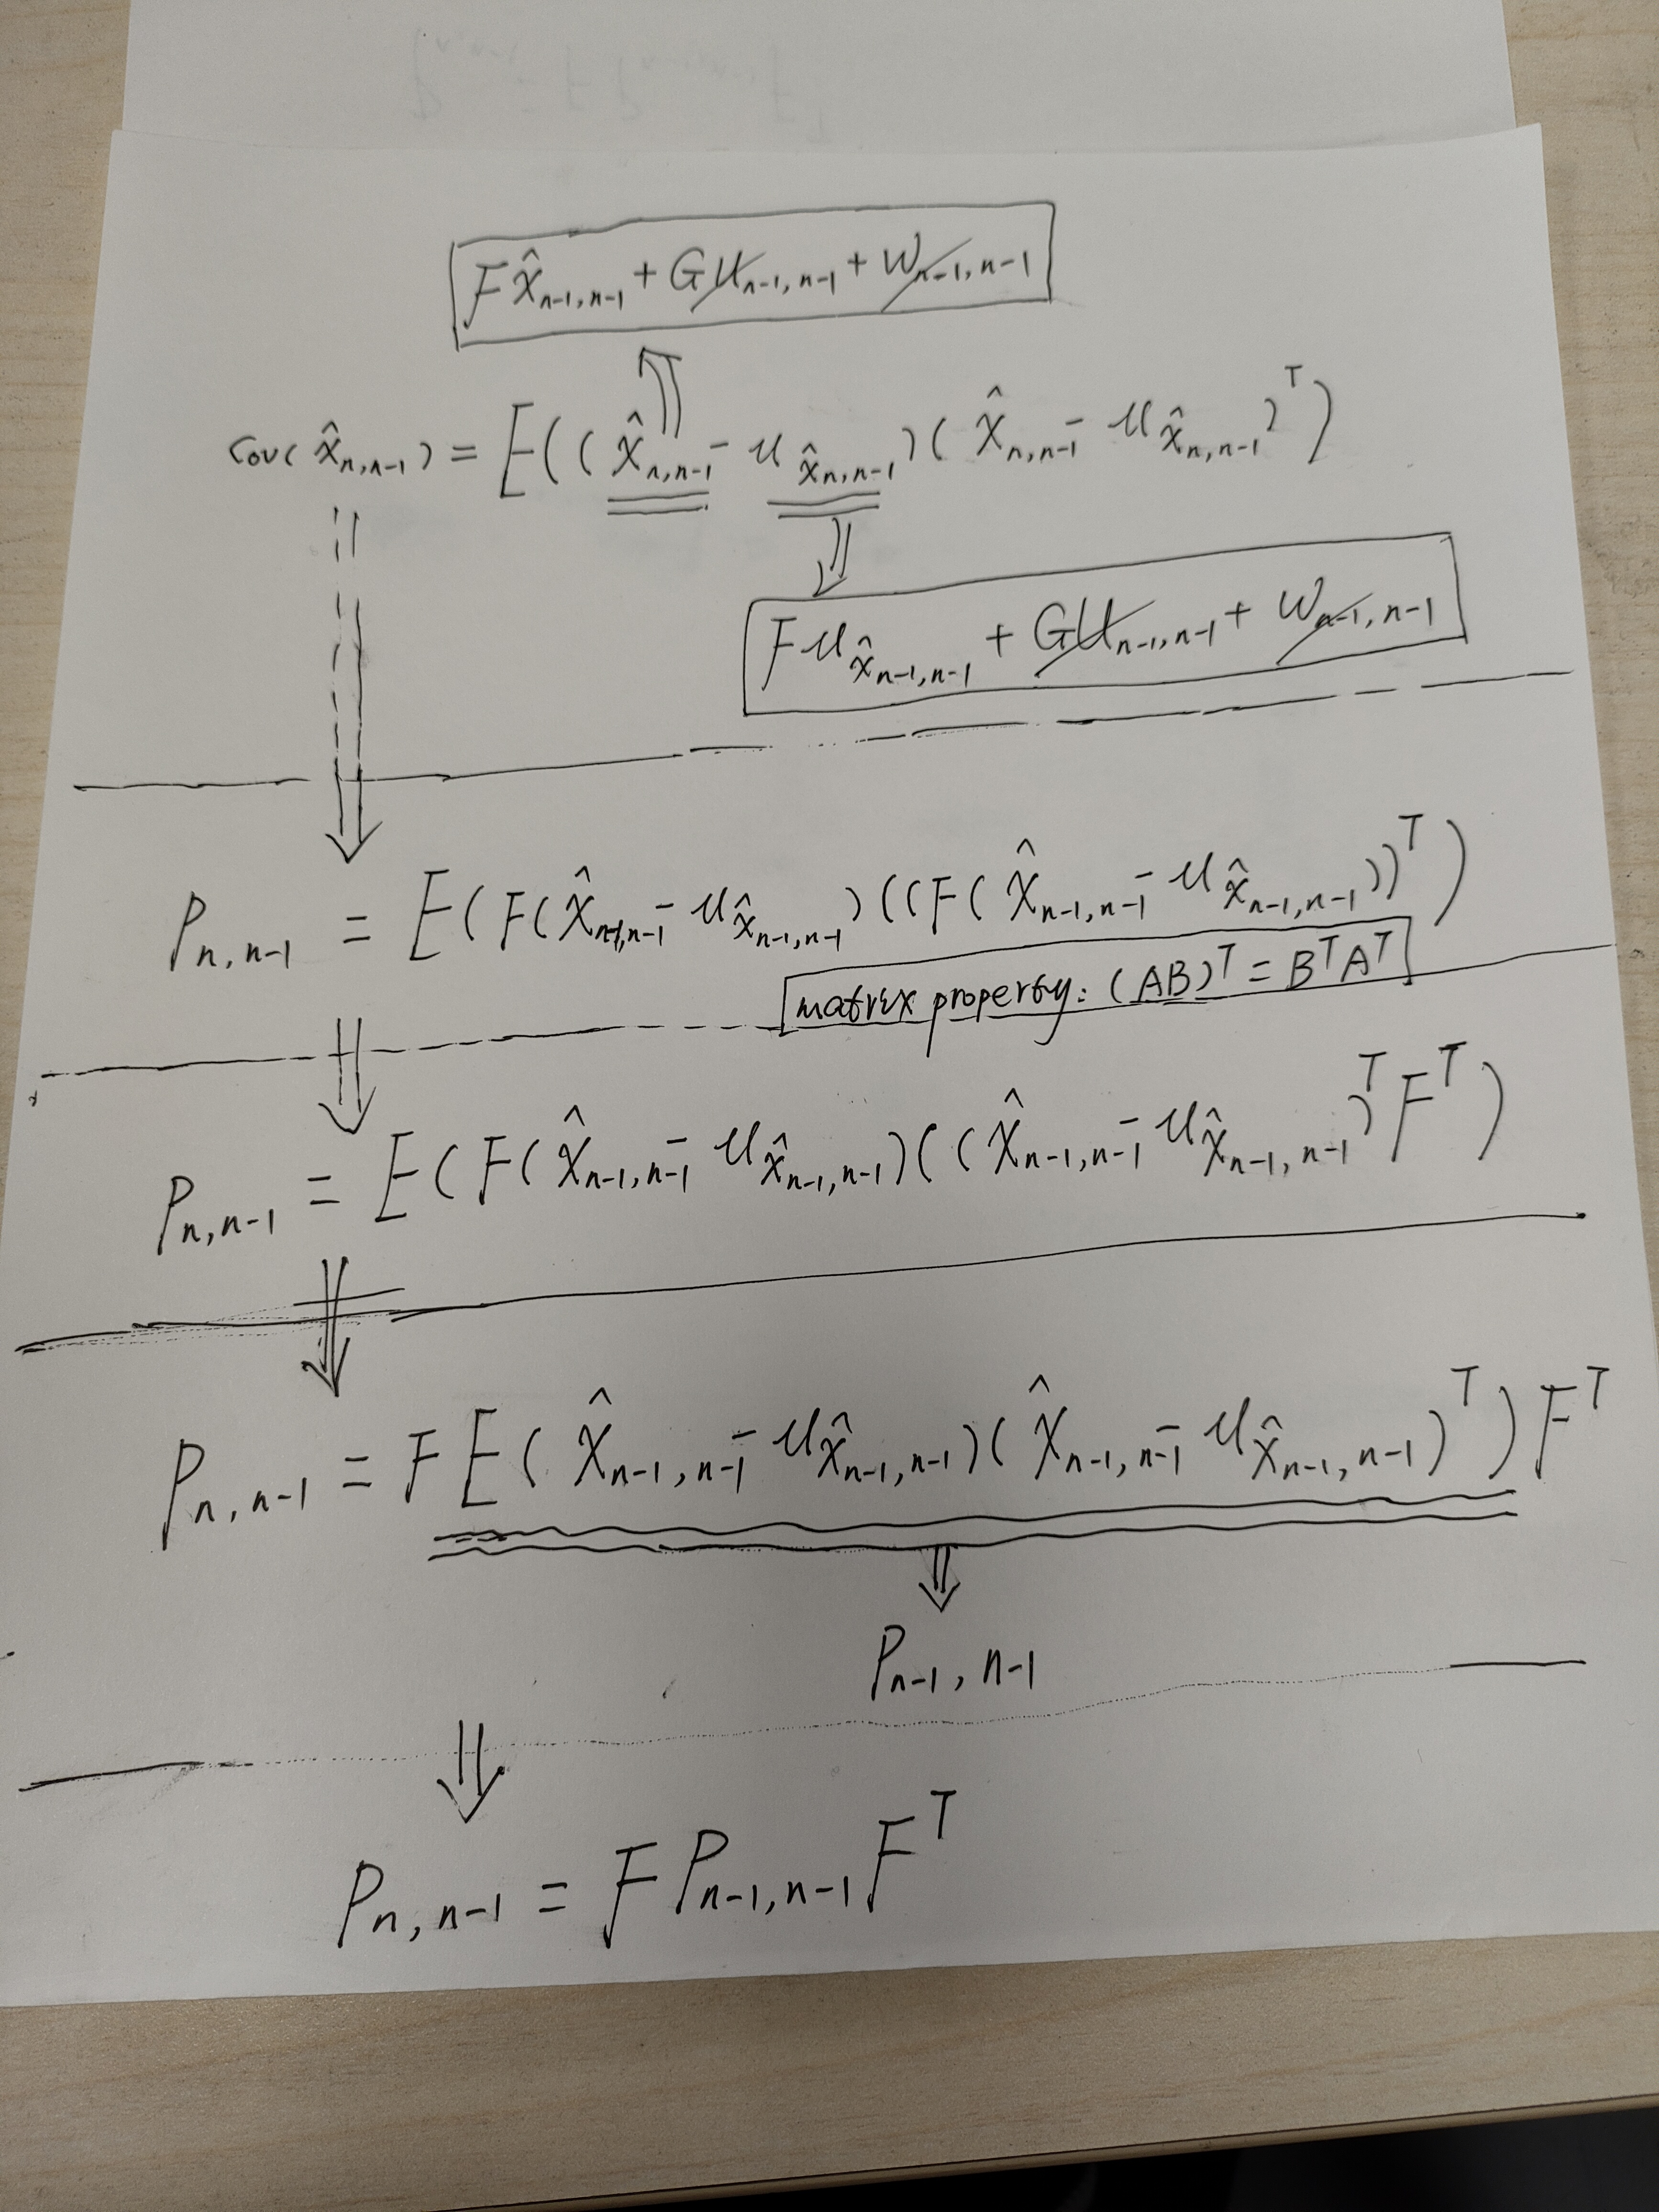
\includegraphics[width=.9\columnwidth]{manual.jpg} 
$$
The Covariance Extrapolation Equation is
\begin{equation} \label{ec-1}
{P}_{n,n-1} = {F}{P}_{n-1,n-1} {F^T}+{Q}
\end{equation}

\subsection{Kalman Gain Equation}
Let's recall our first example (gold bar weight measurement); We made multiple measurements and computed the estimate by averaging.We obtained the following result:
$$
\centering
\includegraphics[width=.9\columnwidth]{gold_10_graph} 
$$
On the above plot, you can see the true values, the estimated values, and measurements vs. the number of measurements.

The differences between the measurements (blue samples) and the true values (green line) are measurement errors. Since the measurement errors are random, we can describe them by variance ( ${\sigma ^2}$ ). The variance of the measurement errors could be provided by the scale vendor or derived by a calibration procedure. The variance of the measurement errors is the measurement uncertainty.

We denote the measurement uncertainty by ${r}$.

The difference between the estimates (the red line) and the true values (the green line) is the estimate error. As you can see, the estimate error becomes smaller and smaller as we make additional measurements, and it converges towards zero, while the estimated value converges towards the true value. We don't know the estimate error, but we can estimate the uncertainty in estimate.

We denote the estimate uncertainty by ${p}$.
I would like to present the intuitive derivation of the Kalman Gain Equation – the third Kalman Filter equation. The mathematical derivation will be shown in the following chapters.

The Kalman Gain (denoted by ${{K}_{n}}$) is the weight given to the current state estimate and the measurements. The Kalman Gain is calculated dynamically for each filter iteration.

The Kalman Gain Equation is the following:\\
$$
&K_{n}=\frac{\text { Uncertainty in Prediction }}{\text { Uncertainty in Prediction + Uncertainty in Measure }} \\
$$
\\
The Kalman Gain is a number between zero and one:
${0 <= {K}_{n} <=1}$ .
Let's rewrite the state update equation:
$$
\hat{x}_{n,n} = \hat{x}_{n,n-1} + {K}_{n}({z}_{n} - \hat{x}_{n,n-1}) = (1-{K}_{n})\hat{x}_{n,n-1} + {K}_{n}{z}_{n}
$$
As you can see, the Kalman Gain (${K}_{n}$) is the measurement weight, and the ($1-{K}_{n}$) term is the weight of the current state estimate.

When the measurement uncertainty is large and the estimate uncertainty is low, the Kalman Gain is close to zero. Hence we give significant weight to the estimate and a small weight to the measurement.

On the other hand, when the measurement uncertainty is low and the estimate uncertainty is large, the Kalman Gain is close to one. Hence we give a low weight to the estimate and a significant weight to the measurement.

If the measurement uncertainty equals the estimate uncertainty, then the Kalman gain equals 0.5. The Kalman gain tells how much the measurement changes the estimate.

The Kalman Filter is optimal since the Kalman Gain minimizes the estimation uncertainty.\\
\textbf{ Kalman Gain Mathematical Derivation}
\\
There are several ways to derive the one-dimensional Kalman Gain equation. I will present the simplest one.

Given the measurement ${z}_{n}$ and the prior estimate ${x}_{n,n-1}$, we are interested to find an optimum combined estimate ${x}_{n,n}$ based on the measurement and the prior estimate.

The optimum combined estimate is actually a weighted mean of the prior estimate and the measurement:
$$
\hat{x}_{n,n} = {k}_{1}{z}_{n} + {k}_{2}\hat{x}_{n,n-1}
$$
Where ${k}_{1}$ and ${k}_{2}$ are the weights of the measurement and the prior estimate.
$$
    {k}_{1} + {k}_{2} = 1
$$
$$
    \hat{x}_{n,n} = {k}_{1}{z}_{n} + (1-{k}_{1})\hat{x}_{n,n-1}
$$
Since we are looking for an optimum estimate, we are interested to minimize ${Var(\hat{x}_{n,n})}$ .
The relation between variances is given by:\\
\\
\begin{aligned}
&Var(\hat{x}_{n,n}) = Var({k}_{1}{z}_{n} + (1-{k}_{1})\hat{x}_{n,n-1})\\
&{P}_{n,n}=Var({k}_{1}{z}_{n})+Var((1-{k}_{1})\hat{x}_{n,n-1})\\
&{P}_{n,n}={k^2}_{1}{R}_{n} + (1-k_1)^2{P}_{n,n-1} \\
\end{aligned}
\\
\\
where:
\begin{itemize}
    \item  ${P}_{n,n}$ is the variance of optimum combined estimate $\hat{x}_{n,n}$.
    \item ${P}_{n,n-1}$ is the variance of the prior estimate $\hat{x}_{n,n-1}$.
    \item ${R}_{n}$ is the variance of the measurement ${z}_{n}$.
\end{itemize}
Since we are looking for an optimum estimate, we are interested to minimize ${p}_{n,n}$.In order to find ${k}_{1}$ that minimizes ${p}_{n,n}$, we differentiate ${p}_{n,n}$ with respect to ${k}_{1}$ and set the result to zero.\\
\\
\begin{array}{c}
\frac{d P_{n, n}}{d k_{1}}=2 k_{1} R_{n}-2\left(1-k_{1}\right) P_{n, n-1} \\
k_{1} R_{n}=P_{n, n-1}-k_{1} P_{n, n-1} \\
k_{1} P_{n, n-1}+k_{1} R_{n}=P_{n, n-1} \\
k_{1}=\frac{P_{n, n-1}}{P_{n, n-1}+R_{n}}\\
\end{array}
\\
\\
We have derived the Kalman Gain! Since the Kalman Gain yields the minimum variance estimate, the Kalman Filter is also called an optimal filter.

And we have other approach to derivd the Kalman Gain.
\\
\\
\begin{aligned}
&Var(\hat{x}_{n,n}) = Var({k}_{1}{z}_{n} + (1-{k}_{1})\hat{x}_{n,n-1})\\
&{P}_{n,n}=Var({k}_{1}{z}_{n})+Var((1-{k}_{1})\hat{x}_{n,n-1})\\
&{P}_{n,n}={k^2}_{1}{R}_{n} + (1-k_1)^2{P}_{n,n-1} \\
\end{aligned}
\\
\\
$$
{f(k_1)} = {k^2}_{1}{R}_{n} + (1-k_1)^2{P}_{n,n-1}-{P}_{n,n}
$$
$$
{f(k_1)} = (R_n+{P}_{n,n-1}){k^2}_{1} - 2{k}_{1}{P}_{n,n-1}-{P}_{n,n}+{P}_{n,n-1}
$$
$$
\centering
\includegraphics[width=.9\columnwidth]{k1} 
$$
Since we are looking for an optimum estimate, we are interested to minimize ${f(k_1)}$.we differentiate ${k}_{1}$ and set the result to zero.\\
\\
$$
\frac{d f(k_1)}{d k_{1}}=0 \\
$$

$$
&K_{n}=\frac{P_{n, n-1}}{P_{n, n-1}+R_{n}} \\
$$
\\

we denoted the measurement by ${z}_{n}$.

The measurement value represents a true system state in addition to the random measurement noise ${v}_{n}$, caused by the measurement device.

The measurement noise variance ${r}_{n}$ can be constant for each measurement - for example, if we have scales that have a precision of 0.5kg (standard deviation). On the other hand, the measurement noise variance rn can be different for each measurement - for example, if we have a thermometer that has precision of 0.5\% (standard deviation). in the latter case, the noise variance depends on the measured temperature.

The generalized measurement equation in matrix form is given by:
$$
{z}_{n} = {H}{x}_{n} + {v}_{n} 
$$
Where:
\begin{itemize}
\item ${z}_{n}$	is a measurement vector.
\item ${x}_{n}$	is a true system state (hidden state).
\item ${v}_{n}$	is a random noise vector.
\item ${v}_{n}$	is an observation matrix.
\end{itemize}
In many cases the measured value is not the desired system state. For example, a digital electric thermometer measures an electric current, while the system state is the temperature. There is a need for a transformation of the system state (input) to the measurement (output).

The purpose of the observation matrix ${H}$ is to convert system state into outputs using linear transformations. The following chapters include examples of the observation matrix usage.\\
\textbf{State Selection}\\
Sometimes certain states are measured while others are not. For example, the first, third and fifth states of a five-dimensional state vector are measurable, while second and fourth states are not measurable:
$$
{z}_{n}=
\left[\begin{array}{ccccc}
1 & 0 & 0 & 0 & 0   \\
0 & 0 & 1 & 0 & 0   \\
0 & 0 & 0 & 0 & 1   \\
\end{array}\right]
\left[\begin{array}{l}
{x}_{1} \\
{x}_{2} \\
{x}_{3} \\
{x}_{4} \\
{x}_{5} \\
\end{array}\right]+
{v}_{n} = \left[\begin{array}{l}
{x}_{1} \\
{x}_{3} \\
{x}_{5} \\
\end{array}\right]+
{v}_{n}
$$
\\
$$
{z}_{n} = {H}{x}_{n} + {v}_{n} \\
$$
\\
The measurement error is given by:
$$
{e}_{n} = ({z}_{n} - H{\hat{x}_{n,n-1}})
$$
The measurement uncertainty is given by:
$$
{r}_{n}=E({e}_{n}{e}_{n}^T)
$$
The Kalman Gain Equation is the following:
\begin{equation} \label{ec-1}
K_{n}=\frac{P_{n, n-1}}{P_{n, n-1}+R_{n}} 
\end{equation}

\subsection{State Update Equation}
The State Update Equation in the matrix form is given by:
\begin{equation} \label{ec-1}
\hat{x}_{n,n}=\hat{x}_{n,n-1} + K_{n}({z}_{n}-H\hat{x}_{n,n-1})
\end{equation}
You should pay attention on the dimensions. If, for instance, the state vector has 5 dimensions, while only 3 dimensions are measurable (the first, third and fifth states):
$$
{x}_{n}=
\left[\begin{array}{l}
{x}_{1} \\
{x}_{2} \\
{x}_{3} \\
{x}_{4} \\
{x}_{5} \\
\end{array}\right]
$$
$$
{z}_{n}=
\left[\begin{array}{l}
{z}_{1} \\
{z}_{2} \\
{z}_{3} \\
\end{array}\right]
$$
The observation matrix would be 3×5 matrix:
$$
{H}=
\left[\begin{array}{ccccc}
1 & 0 & 0 & 0 & 0   \\
0 & 0 & 1 & 0 & 0   \\
0 & 0 & 0 & 0 & 1   \\
\end{array}\right]
$$
\\
The innovation $({z}_{n}-H\hat{x}_{n,n-1})$ yields:\\
\begin{array}{c}
\left(\boldsymbol{z}_{\boldsymbol{n}}-\boldsymbol{H} \hat{\boldsymbol{x}}_{\boldsymbol{n}, \boldsymbol{n}-\mathbf{1}}\right)=\left[\begin{array}{l}
z_{1} \\
z_{3} \\
z_{5}
\end{array}\right]-\left[\begin{array}{ccccc}
1 & 0 & 0 & 0 & 0 \\
0 & 0 & 1 & 0 & 0 \\
0 & 0 & 0 & 0 & 1
\end{array}\right]\left[\begin{array}{l}
\hat{x}_{1} \\
\hat{x}_{2} \\
\hat{x}_{3} \\
\hat{x}_{4} \\
\hat{x}_{5}
\end{array}\right]= \\
\left[\begin{array}{l}
\left(z_{1}-\hat{x}_{1}\right) \\
\left(z_{3}-\hat{x}_{3}\right) \\
\left(z_{5}-\hat{x}_{5}\right) \\
\end{array}\right] \\
\end{array} \\
\\
\\
The Kalman Gain dimensions shall be $5$ * ${3}$.

\subsection{Covariance Update Equation}
The Covariance Update Equation is given by:\\
\begin{equation} \label{ec-1}
\boldsymbol{P}_{n, n}=\left(I-K_{n} H\right) P_{n, n-1}\left(I-K_{n} H\right)^{T}+K_{n} R_{n} K_{n}^{T}
\end{equation}
Where:
\begin{itemize}
\item ${P}_{n,n}$ is the estimate uncertainty(covariance).
\item ${P}_{n,n-1}$ is the prediction uncertainty(covariance).
\item ${K}_{n}$ is the Kalman Gain.
\item ${H}$ is the observation matrix.
\item ${R}_{n,n-1}$ is the measurement uncertainty(covariance).
\item ${I}$ is an Identity matrix.
\end{itemize}










% The minor equations or definitions of variables can be inserted directly in the paragraph line, for example, consider that you want to define a story $\vect{h}_i^n = w_{i-1}. w_{i-2}, \dots, w_{i-n+1}$ associated with a $w_i$ symbol. Note that a simple way to ensure uniformity in the style of the equations is to write the mathematical formulations always in the corresponding environment, that is, using \verb!$a + b$! to write for example $a + b$ (do not write directly as the text a + b). On the other hand, remember that the units of measurement should always be written in \emph{round} format, so that they are not mistaken by variables (for example, $1\,\text{m} = 100\,\text{cm}$ instead of $1m = 100cm$).

% To insert more complex equations or to be referenced, it is recommended to use the equation environments available in the package \verb!amsmath!, noticing that the command \verb!\begin{equation}! automatically enumerate the equations. To write equations without enumerating use \verb!\begin{equation*}! or simply \verb!$$<equation>$$! to get the expression on a separate line, for example $$ \frac{a + b + c}{2} = d. $$ In the case of an enumerated equation, its \emph{tag} must be defined with the command \verb!\label{ec-1}!:

% \begin{equation} \label{ec-1}
%  P_l(w_i|\vect{h}_i^{k}) = \sum_{j=0}^{k-1} \lambda_j \hat{P}(w_i|\vect{h}_i^{j}).
% \end{equation}

% To refer to this equation from the text you must use the command \verb!\eqref{ec-1}!, which automatically places the number of the equation inside parentheses. For example, ``in eq.~\eqref{ec-1} you can see the estimate of the probability of a story from the simple linear combination of lower order stories. '' Remember that the use of \emph{in quotation marks} in \LaTeX\ must be done using the corresponding commands: using \verb!``text''! to get ``text''.

% If your work involves the use of extensive mathematical formulations as in eq.~\eqref{ec-2}, which might not be displayed correctly in the two-column format, you might use an extended float with the command \verb!\begin{figure*}[t]! to arrange the equation in the total width of the page and at the top of the text. The delimiters  $(\mbox)$, $[\mbox]$, $\{\mbox\}$  must be used correctly by the commands \verb!\left* \right*! so that its size automatically adjusts to the mathematical expression. %fiquei confuso com esta parte final%

% \begin{figure*}[!t]
%  \begin{equation}\label{ec-2}
%   b = \left\{\frac{1}{\alpha_1 + 1}\left(x_s - x_i\right)^{\alpha_1+1} + \frac{k}{\alpha_2 + 1}
%   \left[\left(c - x_i\right)^{\alpha_2+1} - \left(x_s - x_i\right)^{\alpha_2+1}\right]
%   + \frac{\beta}{\beta + 1}\left[\left(x_s - x_i\right)^{\alpha_1} - 
%   \left(x_s + x_i\right)^{\alpha_2}\right]\right\}^{-1}.
%  \end{equation}
% \end{figure*}


% \subsection{Figures}

% Figures should be properly referenced using the traditional \LaTeX\ commands, and should never be placed as loose elements within the text. The figure caption is automatically placed using the environment
% \begin{verbatim}
% \begin{figure}[!tb]
%   \centering
%   \includegraphics[<options>]{<file>}
%   \caption{Epigraph} \label{<label>}
% \end{figure}
% \end{verbatim}
% and filling in the corresponding field in \verb!\caption{<>}! (see Fig.~\ref{fig-1}). The figures can be contained in PDF, JPG or PNG files, among others. Within the field \verb![<options>]! you can use the \verb![width=.8\columnwidth]! if it is necessary to adjust the size of the figure. Fig 1 has been set as an example using the factor \verb!.8! .

% \begin{figure}[!tb] 
%  \centering
%  \includegraphics[width=.8\columnwidth]{figura1} 
%  \caption{Outline of the map used indicating the different ways of reinjection and the effect of noise.} \label{fig-1}
% \end{figure}

% Preferably, the figures should be arranged at the beginning or end of a column of text (for which the \texttt{[!tb]} option is used), and in general it is not advisable to arrange the figures on special pages at the end ??from work??. Do not include additional breaks or spaces at the ends of the figures as these are duly defined in the class file. If Cartesian axes are used in the figure, always remember to describe what each axis (labels) corresponds to, with a font of size no smaller than 7 pt for easy reading. To refer to a figure, use the abbreviated form Fig. followed by the \verb!\ref{label}! command, except when it is at the beginning of a paragraph, in which case the whole word should be used.

% \begin{figure*}[!tb] 
%  \centering
%  \includegraphics{figura2.pdf} 
%  \caption{Example of the aliasing that occurs in a grid with $N = 8$ nodes. Both modes ($k = 2$ and $k = 10$) take the same values at the grid points.} \label{fig-2}
% \end{figure*}

% If possible, do not include colors in the graphics, preferably use different types of lines. Also, keep in mind that vectorized graphics provide better electronic and print quality, therefore, insert all graphics with some vectorized format or, if it is a more complex photograph or image, use formats with lossless compression of information (JPG, PNG, TIF, GIF, etc. formats can be configured). To include figures that need to be displayed in the total width of the page, the \verb!\begin{figure*}! environment must be used again, as in the case of Fig.~\ref{fig-2}.

% \subsection{Tables}

% It is preferable that the tables are designed using the \LaTeX\ commands defined for this purpose, and not added as image files as this is detrimental to the quality of the document. However, this option may be acceptable if the insertion is made from a vectorized format that respects the size and style of the typography. The heading of the tables is markedly different at the bottom of the figures. In this case, it is placed above the table, with font size 8 pt and centered paragraph. As in the figures, the tables should be at the beginning or at the foot of a column. The size of the text within the tables should not be smaller than 7 pt or more than 10 pt (the font size used in the general text). An example of this style can be seen in Table~\ref{table-1}.

% \begin{table}[!b]
%  \centering
%   \caption{Final results and relative error reduction (averages over 10 training and test partitions).} \label{table-1}
%  {\small
%  \begin{tabular}{ccccc}
%   \hline
%   \hline
%   \thead{Recognition \\ Errors} & \thead{SER \\ \%} & \thead{WER \\ \%} & \thead{WAER \\ \%} &
%                         \thead{Reduction \\ \% WER} \\
%   \hline
%   \hline
%   Reference & $38.30$ & $7.54$ & $8.53$ & $-$ \\
%   \hline
%   HMM-PASS & $30.55$ & $5.36$ & $6.67$ & $28.91$ \\
%   1-PASS & $25.50$ & $4.76$ & $5.70$ & $36.87$   \\
%   \hline
%   \hline
%  \end{tabular}}
% \end{table}

% \subsection{Bibliographic citations}

% Bibliographic citations will be added through IEEETran system, which uses the \texttt{[x]} format to indicate the references within the text. For this task, the template uses \texttt{Bibtex}, so the references must be included in an external \texttt{*.bib} file (\texttt{References.bib} in this example). In this way, the reference to a bibliographic citation is made with the command \verb!\cite{<label>}!, to obtain for example: ``as seen in the book by \cite{Mitchell2001}''.

% References need to be cited in text. Multiple references are each numbered with separate brackets. When citing a section in a book, please give the relevant page numbers. In text, refer simply to the reference number. Do not use ``Ref." or ``reference" except at the beginning of a sentence: ``Reference [3] shows ... .".

% Reference numbers are set flush left and form a column of their own, hanging out beyond the body of the reference. The reference numbers are on the line, enclosed in square brackets. In all references, the given name of the author or editor is abbreviated to the initial only and precedes the last name. Use them all; use et al. only if names are not given. Use commas around Jr., Sr., and III in names. Abbreviate conference titles.  When citing journals, provide the issue number, page range, volume number, year, and/or month if available. When referencing a patent, provide the day and the month of issue, or application. References may not include all information; please obtain and include relevant information. Do not combine references. There must be only one reference with each number. If there is a URL included with the print reference, it can be included at the end of the reference.

% Other than books, capitalize only the first word in a paper title, except for proper nouns and element symbols.


% In the section of the Bibliography the style for the different types of bibliographic citations consists of:

% \begin{itemize}
%  \item Book: Authors, year in parentheses. Title in italics, editorial, place of publication \cite{Alarcos1999}. It is included using the \texttt{@book} option in the references file.
% %
%  \item Book chapter: Authors, year in parentheses. Chapter title in quotes. In: book title in italics of the book, pages, editorial, place of publication \cite{Mitchell2001}. It is included with the \texttt{@inbook} field in the reference file.
% %
%  \item Article in periodic magazine: Authors, year in parentheses. Title of the article in quotation marks, name of the magazine in italics, volume, number in parentheses, pages \cite{ArslanHansen1996, WangEtAl2015}. It is included using the \texttt{@article} option.
% %
%  \item Conferences: Authors, year in parentheses. Article title in quotes. In: title of the memoirs or of the event in italics, editorial of the publication of the memoirs, place of publication, pages \cite{BarkovaJouvet1999}. It is included with the \texttt{@inproceedings} field in the reference file.
% %
%  \item Website: Authors, year in parentheses. Title of the article in quotes, taken from <URL>, query date of the web page in parentheses \cite{CFDwebpage}. It is included with the \texttt{@webpage} option.
% %
%  \item Technical report: Authors, year in brackets. Title of the report in quotes, ``Report Nº'', institution in italics, place of publication \cite{NACA460}. It is included using the \texttt{@techreport} field.
% %
%  \item Thesis, thesis or final work: Authors, year in parentheses. Title in italics, type of work. Institution, place of presentation \cite{Krause2014}. It is included using the \texttt{@thesis} field in the reference file.
% %
%  \item Manual or technical report: Authors, year in parentheses. Title in italics, organization or institution, place of publication \cite{Indura2010}. It is included with the \texttt{@manual} option.
% %
%  \item Other forms of communication: to reference other forms of communication, you must always specify the author or entity, the year and the way in which the communication was made. You can optionally include a title and an explanatory note. These types of references are included using the \texttt{@other} field.
% \end{itemize}

% The bibliographic references section is labeled as ``References'' (or with its equivalent depending on the chosen language) and has a particular style for the paragraph, where the indentation is eliminated and the font size is reduced (fixed at 8 pt ). References should be showed in alphabetical order taking into account the last name of the first author, regardless of the order of appearance in the text. Remember that all references included in the bibliography section must be duly cited in the text.

% To fully satisfy the definitions established for the bibliography and facilitate subsequent editing and publishing tasks, it is strongly recommended to use the reference style provided, including bibliography by the command
% \begin{verbatim}
%  \insertbibliography{<file.bib>} 
% \end{verbatim}
% at the end of manuscript.

% \subsection{Other general recommendations}

% Define properly each of the acronyms used describing their meaning the first time they appear in the text. For example, ``such a relationship is known as the mass ratio (RGM)''. Once defined, always use the acronym instead of the full term. Remember to define each of the symbols that appear in the mathematical expressions and do not forget to clarify the notation used when using special or unusual mathematical operators. The use of capital letters should be made according to the general conventions, that is, at the beginning of a sentence after a period, in proper names, in acronyms, etc., and in titles according to what is defined in the work format. If in doubt, contact ajceam@gmail.com.


% \section{Conclusions}

% The conclusions should present a review of the key points of the article with special emphasis on the analysis and discussion of the results that were made in the previous sections and in the applications or extensions of them. You should not reproduce the summary in this section or repeat paragraphs already included in another sections of the work.

% \section{Acknowledgment}

% If there are acknowledgments, references to research projects, or work-financing entities, these should be included in the ``Acknowledgments'' section afterward the conclusions of the work. Check the following: if the place the names and/or codes corresponding to research projects, institutions, financing programs, etc., involved in the work.

% % Include appendices (if necessary)
% \appendix
% \section{Appendices}

% In some situations it is convenient to include a section of appendices with their corresponding subsections.

% \subsection{Demonstrations}

% Demonstrations might be included in the main text provided that their extension and complexity do not distract the reader from the most relevant contents of the work. Otherwise, it is recommended to provide only the final results in the text including the demonstrations in an appendix at the end of the work.

% \subsection{Algorithms}

% In the same way as in the previous case, the algorithms are not too extensive, they might be included within the main body of the work, otherwise they should be arranged in an appendix at the end of the work.

% \subsection{Other data}

% The inclusion of technical details, accessory measurements, data tables or other information relevant to the work should be done in the form of an appendix when justified, otherwise they can be included directly in the main body of the text when reference is made to the same.

%README
\section{README}
\begin{itemize}
\item Love life, love technology, pay attention to the accumulation of professional knowledge.
\item Creator who is willing to share, cheerful and has a good team atmosphere.
\item Positive work attitude, focused attention and responsibility.
\item Experienced software engineer who constantly seeks out innovative solutions to everyday problems.
\item Have honed my analytical thinking and collaboration skills, and love working teams.
\end{itemize}
\section{Miscellaneous}
\item GitHub: https://github.com/pengfeinie
\item Home: https://pengfeinie.github.io/
\item Blog: https://blog.csdn.net/pfnie

% Include references
\insertbibliography{References}
1.\quad https://www.kalmanfilter.net/default.aspx
\end{document}
